\documentclass[fleqn]{tcdl}

\title{Gramáticas y Parsers, Primera Parte}
\author[1]{Ernesto Bossi}
\affil[1]{Profesor}

\begin{document}

\flushbottom
\maketitle
\thispagestyle{empty}

\section*{Introducción}
\fontsize{11}{14}\selectfont

En la compilación o interpretación de un lenguaje existen distintas etapas, desde que nosotros tenemos nuestro input hasta que generamos una salida que nos sirve la para ejecución ya sea instrucciones de máquina u otro tipo de instrucciones que nos permitan de alguna manera interpretar esas instrucciones y poder tener un resultado de la entrada computacionalmente.
\\\\

\begin{figure}[h]
\captionsetup{type=figure}
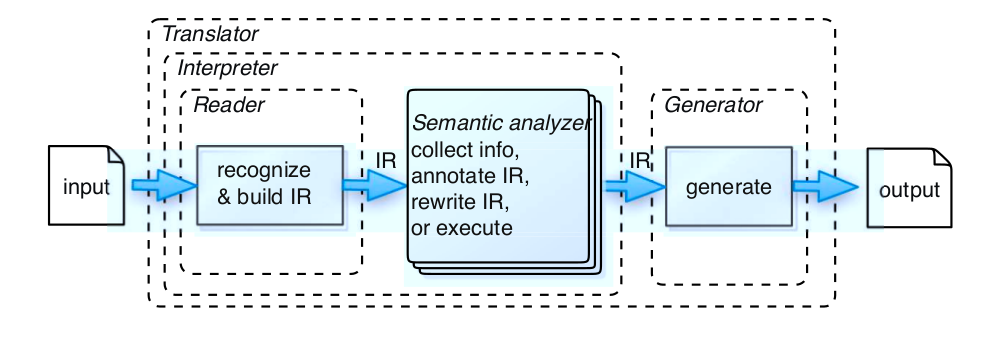
\includegraphics[width=\textwidth]{etapas.png}
\caption{\label{fig:comp_basic}Etapas de compilación.}
\end{figure}

\begin{itemize}
\item Lector: que genera una estructura a partir de un input que es texto en genera, aunque puede ser a veces binario. Esta estructura la llamaremos IR.
\item Generador: recorre la estructura y genera una salida a partir de este que puede serla salida misma de un compilador.
\item Traductor: Un traductor leer una entrada de texto o binario y la traduce a otra salida que puede ser una traducción de un lenguaje a otro. Es un lector combinado con un generador. Ej. un profiler, refactor engine, etc.
\item Intérprete: Un interprete lee, decodifica y ejecuta instrucciones desde simples cálculos hasta operaciones mas complejas, podemos ver esto en entornos como el de Ruby y Python cuyo interprete ejecuta un output final que es bytecode.
\end{itemize}

Existen muchos tipos de representaciones intermedias, la que nos interesa en particular por el momento es generar una construcción en forma de árbol llamada AST (Abstract syntax Tree). El AST sería un IR? No exactamente, si bien muchas IR son similares a los AST, los IR se refiere más al concepto de tener una representación de datos que está más asociada a una máquina abstracta en la que se realizará el análisis semántico, junto con las optimizaciones antes de pasar a la etapa de code generation. Nos interesa tener una construcción abstracta ya que nos permitirá trabajar con ella, y contendrá más información sobre el input que recibimos y no solamente texto. De esta manera será más fácil de saber el orden de ejecución y la información de cada uno de los nodos. Porqué vemos un AST como primer tipo de construcción abstracta? Porque es lo más simple para trabajar, si bien hay otro tipo de construcciones como ASG que nos permitirán trabajar más cómodo con lenguajes más complejos.

Por ej. si tenemos una expresión como this.x = y el AST que se forma una vez parseada la misma es:

\begin{figure}[h]
\captionsetup{type=figure}
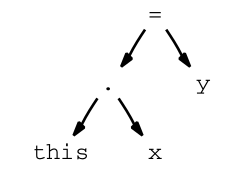
\includegraphics[width=200pt]{ast1.png}
\caption{\label{fig:comp_basic}Ejemplo de un AST.}
\end{figure}

Aquí se puede ver que cada uno de los nodos del árbol representa un miembro de la expresión ya sea un identificador como x o y ó operadores como . o =. Como se remarcó antes estos nodos no solo tendrá definido el texto de entrada sino a que tipo pertenecen y el orden de evaluar la expresión dependerá de cómo es la estructura del AST, en este caso el orden de evaluación es de izquierda a derecha y de abajo hacia arriba. Existen distintos algoritmos para armar el AST y recorrer estos, luego pasaremos más links ya que nuestro objetivo al menos es la de aprender el paso para armar estas expresiones.

Volviendo al proceso que veremos hoy, el pipeline o pasos que veremos de la compilación son los siguientes:

\begin{figure}[h]
\captionsetup{type=figure}
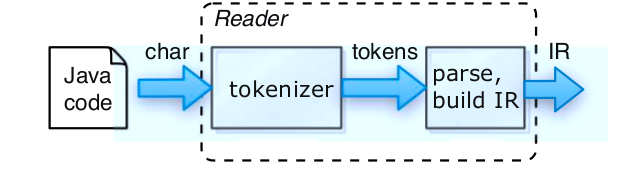
\includegraphics[width=\textwidth]{frontend1.png}
\caption{\label{fig:comp_basic}Etapas de front end de un compilador.}
\end{figure}

\end{document}